\documentclass[mathNotesPreamble]{subfiles}
\begin{document}
%\relscale{1.4} %TODO
\section{16.2: Double Integrals over General Regions}

  In this section, we consider double integrals over non-rectangular regions. For instance, my domain for $x$ and $y$ can be constrained where $a\leq x\leq b$ and $g(x)\leq y\leq h(x)$:
  \vspace*{\stretch{1}}
  \begin{center}
    \begin{tikzpicture}
      \begin{axis}[
        grid style={line width=0.35pt, draw=gray!75},
        axis lines=center,
        axis line style={black,->},
        xmin=-1, xmax=6,
        ymin=-1, ymax=7,
        xtick={1,4},
        xticklabels={$a$,$b$},
        ymajorticks=false,
        enlargelimits={abs=0.75},
        ticklabel style={font=\normalsize,inner sep=0.5pt,fill=white,opacity=1.0, text opacity=1},
        xlabel=$x$, xlabel style={at={(ticklabel* cs:1)},anchor=north west},
        ylabel=$y$, ylabel style={at={(ticklabel* cs:1)},anchor=south west},
        every axis plot/.append style={line width=0.95pt, color=ClemsonPurple, samples=100}
        ]
        \addplot[->, name path=A] expression[domain=-0.5:6]{(2*x/3-2)^2}
          node[right, black, pos=0.7] {$g(x)$};
        \addplot[->, name path=B] expression[domain=-0.5:6]{6-(x/2-1)^2}
          node[right, black, pos=0.55] {$h(x)$};
        \addplot[fill=ClemsonOrange!55] fill between[of=A and B, soft clip={domain=1:4}];
      \end{axis}
    \end{tikzpicture}
  \end{center}
  \vspace*{\stretch{1}}

  \begin{thmBox*}[Theorem 16.2: Double Integrals over Nonrectangular Regions]
    Let $R$ be a region bounded below and above by the graphs of the continuous functions $y=g(x)$ and $y=h(x)$, respectively, and by the lines $x=a$ and $x=b$. If $f$ is continuous on $R$, then
      \[\iint\limits_R f(x,y)\,dA=\int_a^b \int_{g(x)}^{h(x)} f(x,y)\,dy\,dx.\]
    Let $R$ be a region bounded on the left and right by the graphs of the continuous functions $x=g(y)$ and $x=h(y)$, respectively, and the lines $y=c$ and $y=d$. If $f$ is continuous on $R$, then
      \[\iint\limits_R f(x,y)\,dA=\int_c^d\int_{g(y)}^{h(y)}f(x,y)\,dx\,dy.\]
  \end{thmBox*}
  \pagebreak

  \begin{ex*}
    Consider the surface generated by the function $f(x,y)=3xy$. Find the volume of the solid generated by $f(x,y)$ over the region bounded by $2x^2$ and $3-x^2$.
  \end{ex*}
  \begin{flushright}
    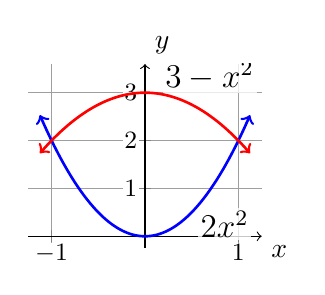
\begin{tikzpicture}
      \begin{axis}[
        grid=both, %major,minor
        grid style={line width=0.35pt, draw=gray!75},
        axis lines=center,
        axis line style={black,->},
        xmin=-1.25, xmax=1.25,
        ymin=-0.25, ymax=3.6,
        ticklabel style={font=\small,inner sep=0.5pt,fill=white,opacity=1.0, text opacity=1},
        xlabel=$x$, xlabel style={at={(ticklabel* cs:1)},anchor=north west},
        ylabel=$y$, ylabel style={at={(ticklabel* cs:1)},anchor=south west},
        every axis plot/.append style={line width=0.95pt, color=blue, samples=100},
        width=0.375\linewidth,
        ]
        \addplot[<->] expression[domain=-1.125:1.125]{2*x^2} 
          node[black, pos=0.65, below right, fill=white, opacity=0.775, text opacity=1, inner sep=1pt, font=\large] {$2x^2$};
        \addplot[<->] expression[domain=-1.125:1.125, red]{3-x^2} 
          node[black, pos=0.55, above right, fill=white, opacity=0.775, text opacity=1, inner sep=1pt, font=\large] {$3-x^2$};
      \end{axis}
    \end{tikzpicture}

    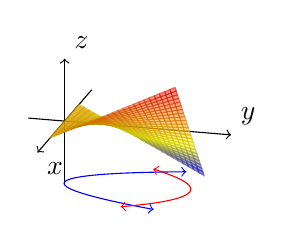
\begin{tikzpicture}
      \begin{axis}[
        axis lines=center,
        axis line style={black,->},
        xmin=-1.125, xmax=1.125,  xmajorticks=false,
        ymin=-0.125, ymax=3.25,  ymajorticks=false,
        zmin=-8.5,  zmax=8.5,  zmajorticks=false,
        enlargelimits={abs=0.75},
        ticklabel style={font=\normalsize,inner sep=0.5pt,fill=white,opacity=1.0, text opacity=1},
        xlabel=$x$, xlabel style={at={(ticklabel* cs:1)},anchor=north west},
        ylabel=$y$, ylabel style={at={(ticklabel* cs:1)},anchor=south west},
        zlabel=$z$, zlabel style={at={(ticklabel* cs:1)},anchor=south west},
        width=0.4\linewidth,
        view={105}{27.5},
        ]
        \addplot[<->] expression[domain=-1.125:1.125, blue]{2*x^2};
        \addplot[<->] expression[domain=-1.125:1.125, red]{3-x^2};
        \addplot3[surf, opacity=0.5, domain=-1:1, y domain=0:3] {3*x*y};
      \end{axis}
    \end{tikzpicture}
  \end{flushright}
  \vspace*{\stretch{1}}
  \pagebreak

  \begin{ex*}
    Find the area under $f(x,y)=\frac{1}{x}+1$ over the region formed by the lines $x=2$, $y=1+x$, and $y=5-x$.
  \end{ex*}
  \begin{flushright}
    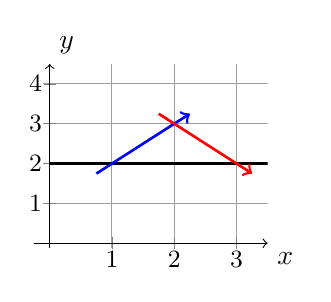
\begin{tikzpicture}
      \begin{axis}[
        grid=both, %major,minor
        grid style={line width=0.35pt, draw=gray!75},
        axis lines=center,
        axis line style={black,->},
        xmin=-0.25, xmax=3.5,
        ymin=-0.125, ymax=4.5,
        ytick={1,2,3,4},
        ticklabel style={font=\small,inner sep=0.5pt,fill=white,opacity=1.0, text opacity=1},
        xlabel=$x$, xlabel style={at={(ticklabel* cs:1)},anchor=north west},
        ylabel=$y$, ylabel style={at={(ticklabel* cs:1)},anchor=south west},
        every axis plot/.append style={line width=0.95pt, color=blue, samples=100},
        width=0.375\linewidth,
        ]
        \addplot[-, line width=1.05pt] expression[domain=0:3.5, black]{2};
        \addplot[->] expression[domain=0.75:2.25, blue]{1+x};
        \addplot[->] expression[domain=1.75:3.25, red]{5-x};
      \end{axis}
    \end{tikzpicture}

    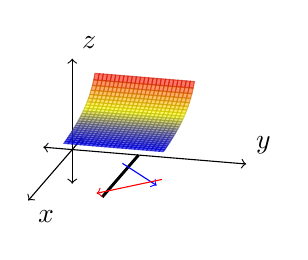
\begin{tikzpicture}
      \begin{axis}[
        axis lines=center,
        axis line style={black,<->},
        xmin=-0.25,  xmax=3.5,  xmajorticks=false,
        ymin=-0.125, ymax=4.5,  ymajorticks=false,
        zmin=0,      zmax=1.25,  zmajorticks=false,
        enlargelimits={abs=0.75},
        ticklabel style={font=\normalsize,inner sep=0.5pt,fill=white,opacity=1.0, text opacity=1},
        xlabel=$x$, xlabel style={at={(ticklabel* cs:1)},anchor=north west},
        ylabel=$y$, ylabel style={at={(ticklabel* cs:1)},anchor=south west},
        zlabel=$z$, zlabel style={at={(ticklabel* cs:1)},anchor=south west},
        width=0.4\linewidth,
        view={105}{27.5},
        ]
        \addplot3[surf, opacity=0.6, domain=1:4, y domain=1:4] {1/x+1};
        \addplot[-, line width=1.05pt] expression[domain=0:3.5, black]{2};
        \addplot[->] expression[domain=0.75:2.25, blue]{1+x};
        \addplot[->] expression[domain=1.75:3.25, red]{5-x};
      \end{axis}
    \end{tikzpicture}
  \end{flushright}
  \vspace*{\stretch{1}}
  \pagebreak

  \begin{ex*}
    Find the volume of the tetrahedron in the first octant bounded by the plane $z=c-ax-by$ and the coordinate planes ($x=0$, $y=0$, and $z=0$). Assume $a$, $b$, and $c$ are positive real numbers.
  \end{ex*}
  \vspace*{\stretch{1}}
  \pagebreak

  \begin{ex*}
    For the following problems, reverse the order of integration
  \end{ex*}
  \begin{tasks}[after-item-skip=\stretch{1}, label=\textbullet](1)
    \task 
      $\displaystyle \int_{0}^{2} \int_{0}^{2x} f(x,y)\,dy\,dx$
    \task 
      $\displaystyle \int_{0}^{1} \int_{x^3}^{\sqrt{x}} f(x,y)\,dy\,dx$
    \task 
      $\displaystyle \int_{-3}^{4} \int_{2x^2}^{2x+24} f(x,y)\,dy\,dx$
  \end{tasks}
  \vspace*{\stretch{1}}
  \pagebreak

  \begin{ex*}
    Find the volume between $f(x,y)=5-y$ and $g(x,y)=1+x^2$ over the region $R=\set{(x,y): 0\leq y\leq 4-x^2,\ -2\leq x\leq 2}$.
  \end{ex*}
  \begin{flushright}
    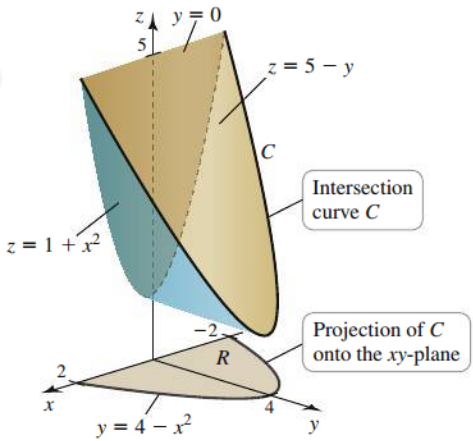
\includegraphics[width=0.3\linewidth]{images/briggs_16_02/fig16_23}
  \end{flushright}
  \vspace*{\stretch{1}}
  \pagebreak

  \begin{thmBox*}[Areas of Regions by Double Integrals]
    Let $R$ be a region in the $xy$-plane. Then
      \[\textnormal{area of } R=\iint\limits_R dA.\]
  \end{thmBox*}

  \begin{ex*}
    Find the area of the region $R$ bounded by $y=x^2$, $y=6-x$, and $y=6+5x$.
  \end{ex*}

  \pagebreak
  
\end{document}
